\documentclass{article}
\usepackage{polyglossia}
\usepackage[a4paper]{geometry}
\usepackage{mathtools, amssymb, amsfonts}
\usepackage{amsthm}
\usepackage{fontspec}
\usepackage[backend=biber]{biblatex}
\usepackage[vargreek-shape=unicode]{unicode-math}

\setmainfont{STIX}

\usepackage{titling}
\usepackage{float}
\usepackage{listings}
\usepackage{graphicx}
\usepackage[hidelinks]{hyperref}
\usepackage{caption,subcaption}
\usepackage{tikz}
\usepackage[locale = FR, exponent-product = \cdot, inter-unit-product = .]{siunitx}
\usetikzlibrary{shapes,calc,angles,decorations.markings}
\usepackage[shortlabels]{enumitem}
\usepackage{comment}

\setdefaultlanguage{french}
\frenchspacing

%% Math commands
%\renewcommand{\vec}[1]{\symbbf{#1}}
\newcommand{\vv}[1]{\symbf{#1}}
%\renewcommand\epsilon\varepsilon
%\renewcommand\phi\varphi
\newcommand{\N}{\mathbb N}
\newcommand{\Z}{\mathbb Z}
\newcommand{\R}{\mathbb R}
\newcommand{\Q}{\mathbb Q}
\newcommand{\CC}{\mathbb C}
\newcommand{\K}{\mathbb K}
\DeclarePairedDelimiter{\abs}{\lvert}{\rvert}
\DeclarePairedDelimiter{\norm}{\lVert}{\rVert}

%% Math environments
\theoremstyle{definition}
\newtheorem{exo}{Exercice}

\theoremstyle{remark}
\newtheorem*{rap}{Rappel}
\newtheorem*{rem}{Remarque}

%% Titling configuration
\pretitle{\begin{center}\LARGE\textsf }
\title{Électrostatique}
\posttitle{\par\end{center}\vspace{-1.2em}}

\preauthor{}
\author{}
\postauthor{}

\date{\today}

\begin{document}
\maketitle


\section{Notion de charge électrique}

\subsection{Généralités}

La \textit{charge} est, comme la masse, une grandeur permettant de décrire les propriétés physique de la matière. Ici, il s'agit des propriétés concernant son comportement lorsqu'elle est plongée dans un champ électromagnétique (un champ électrique seul, un champ magnétique seul, des ondes radios, la lumière...). Son unité est le \textit{coulomb} (C).

La charge est une caractéristique particulièrement pertinente pour les particules subatomiques, telles que les électrons, protons, muons... La plus petite charge possible pour la plupart de ces particules, appelée \textit{charge fondamentale}, est $e= \SI{1.6e-19}{\coulomb}.$

\vspace{1em}
\fbox{
\parbox[c]{0.94\textwidth}{
\textbf{\textsf{Note historique}} La charge électrique est découverte par les Grecs de l'Antiquité, qui remarquent que les petits boutons d'ambre ornant leurs habits, après avoir frotté avec ceux-ci, se mettent à attirer des petits objets tels que des cheveux. En frottant suffisamment, ils observent même la production d'une étincelle.
}}

\vspace{1em}

Les charges ont un signe: négatif ou positif. Les électrons portent une charge négative de $-e$, les protons une charge positive de $+e$. Dans l'exemple des boutons d'ambre des Grecs, ceux-ci portent une charge négative puisque le fait de les frotter arrache des électrons à la surface contre laquelle ils frottent.

Encore des exemples : lorsque vous enlevez votre pull ou que vous vous peignez ou brossez les cheveux, vous entendez un léger craquement, qui peut même s'accompagner, à luminosité faible, de la présence d'étincelles.

\subsection{Charge d'un système de particules}

Étant donné un système de $N$ particules portant des charges $q_1,\ldots,q_N$, la charge totale du système formé est 
\[Q = q_1+\cdots+q_N.\]

On dit que le système est \textit{électriquement neutre} si $Q=0$. Un système de particules portant chacune des charges électriques différentes peut donc être globalement électriquement neutre.

\paragraph{Quelques exemples.} \begin{itemize}
	\item Les molécules sont globalement neutres, alors qu'une molécule telle que l'eau peut porter des charges partielles, dues à la forte électronégativité de l'atome d'oxygène. 

\begin{figure}[H]	
	\centering
    \begin{tikzpicture}
    \tikzset{dot/.style={circle,fill,inner sep=2pt}};
	\node (H1) at (-0.65,-0.8) [dot,label={below left:H},label={above left:$+\delta e$}]{};
	\node (H2) at (0.65,-0.8) [dot,label={below right:H},label={above right:$+\delta e$}]{};
	\node (O) at (0,0) [dot,label={left:O},label={above right:$-2\delta e$}]{};	
	\draw (H1) -- (O) -- (H2);
	\end{tikzpicture}
	\caption{La molécule d'eau est globalement électriquement neutre, mais chaque atome porte une charge partielle.}
\end{figure}

\begin{rap}
	L'électronégativité est la tendance d'un élément à attirer vers lui et s'accaparer, en quelque sorte, les électrons mis en jeu lors d'une liaison covalente. Le rapport des électronégativités entre les éléments en jeu dans une liaison covalente détermine si l'un d'entre eux va remporter une charge partielle, et le cas échéant c'est l'élément le plus électronégatif. Selon l'échelle de \textsc{Pauling}, les éléments les plus électronégatifs sont ceux qui se trouvent vers le haut et vers la droite du tableau périodique des éléments (hormis les gaz nobles). Ainsi, l'oxygène n'est devancé que par le fluor ($\mathrm{F}$) en terme d'électronégativité.
\end{rap}

\item Le sel, cristal ionique de formule $\mathrm{NaCl}$, composé des ions chlorure $\mathrm{Cl}^{-}$ et sodium $\mathrm{Na}^+$, est globalement neutre, même si chaque ion composant chaque maille de ce cristal est électriquement chargé.

\begin{figure}[h]
	\centering
	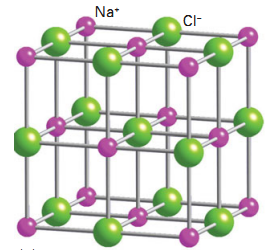
\includegraphics[width=0.36\textwidth]{parts/electrostat/sel_cristal.png}
	\caption{La structure cristalline du sel. Les ions chlorure et sodium sont arrangés dans un motif cubique}
\end{figure}

\begin{rap} Un cristal est un solide dont les constituants (atomiques, ioniques, moléculaires) sont arrangés dans une structure régulière, dans le sens où il existe un arrangement de base, un motif, appelé \textit{maille}, tel que le solide soit en fait un grand réseau où ce motif se répète à l'identique. D'autres exemples sont la neige, le sucre, la fibre de carbone.
\end{rap}

\end{itemize}

\section{Interaction électrostatique}

\subsection{Généralités}

Lorsque deux corps chargés électriquement sont mis en présence, comme un bouton d'ambre chargé et des cheveux, un peigne fraîchement sorti de ceux-ci et un filet d'eau, un pull et un ballon de baudruche, on observe les effets d'une force. En effet, ils se rapprochent (interaction \textit{attractive}) ou s'éloignent (interaction \textit{répulsive}).

Ce comportement est dû au fait que la présence de charges modifie les propriétés de l'espace en créant un \textit{champ électrique}, qui confère à chaque point de l'espace une direction privilégiée dans laquelle orienter les particules chargées et une intensité avec laquelle le faire. Ainsi, une charge qui se retrouve en présence d'une autre est happée par les effets du champ électrique crée par cette dernière.

Le \textit{champ électrique} est un champ vectoriel, c'est-à-dire une fonction d'une variable vectorielle (la position) à valeurs vectorielles (la direction et l'intensité du champ). On le note, classiquement, $\vv{E}$. La situation électrostatique correspond au cas où le champ électrique $\vv{E}$ est indépendant du temps.

L'électrostatique << classique >> (par opposition aux contextes de la théorie de la relativité d'\textsc{Einstein} ou la mécanique quantique de \textsc{Planck}, \textsc{Hilbert}, \textsc{Schrödinger}) est régi par les équations de \textsc{Maxwell} (1831-1879). 


La force exercée par un champ électrique $\vv{E}$ sur une particule de charge $q$ est donnée par
	\[ \vv{F}_\mathrm{él} = q\vv{E}. \]

\subsection{Champ électrique créé par une charge ponctuelle}

Pour le cas d'une charge ponctuelle $q$ située en l'origine, les équations de \textsc{Maxwell} conduisent à la solution
	\[ \vv{E}(\vv{r}) = \frac{1}{4\pi\epsilon_0}\frac{q}{\norm{\vv{r}}^3}\vv{r} \]
où $\epsilon_0\approx\SI{8.854e-12}{\farad\per\meter}$ est la permittivité électrique du vide (sa tendance à laisser passer les champs électriques). Le champ est donc \textit{radial} et ne dépend que de la distance $r=\norm{\vv{r}}$ : $\vv{E} = E(r)\vv{e}_r$, et pour $r = OM$ on retrouve la formule familière
	\[
    E = \frac{1}{4\pi\epsilon_0}\frac{q}{{OM}^2}.
    \]

\begin{figure}[h]
	\centering
	\begin{subfigure}[b]{0.44\textwidth}
		\begin{tikzpicture}
		\tikzset{dot/.style={circle,fill,inner sep=2pt}};
		\tikzset{->-/.style={decoration={
					markings,
					mark=at position #1 with {\arrow{>}}},postaction={decorate}}}
		
		\clip (-3.2,-1.5) rectangle (3.2,1.5);
		\foreach \a in {0,30,60,90,120,150,180,210,240,270,300,330}
		\draw [->-=0.45,color=blue!70,thick] (0,0)--(\a:3.2);
		
		\node (ch) at (0,0) [dot,label={[label distance = 10pt]-3:$q$}]{};
		\end{tikzpicture}
		\caption{Champ créé par une charge positive $q>0$. Les lignes de champ sont orientées vers l'extérieur: le champ est \textit{centrifuge}.}
	\end{subfigure}\qquad
	\begin{subfigure}[b]{0.44\textwidth}
		\begin{tikzpicture}
		\tikzset{dot/.style={circle,fill,inner sep=2pt}};
		\tikzset{->-/.style={decoration={
					markings,
					mark=at position #1 with {\arrow{>}}},postaction={decorate}}}
		
		\clip (-3.2,-1.5) rectangle (3.2,1.5);
		\foreach \a in {0,30,60,90,120,150,180,210,240,270,300,330}
		\draw [->-=0.57,color=red!70,thick] (\a:3.2)--(0,0);
		
		\node (ch) at (0,0) [dot,label={[label distance = 10pt]93:$q$}]{};
		\end{tikzpicture}
		\caption{Champ créé par une charge négative $q<0$. Les lignes de champ sont orientées vers l'origine : le champ est \textit{centripète.}}
	\end{subfigure}
    \caption{Champ électrique créé par une charge ponctuelle $q$.}
\end{figure}

\begin{rap}
	On a $k=\dfrac{1}{4\pi\epsilon_0}=\SI{9.0e9}{\meter\per\farad}.$
\end{rap}

Ainsi, étant donnée une deuxième particule de charge $q_0$ en un point $\vv{r}$, la force électrostatique exercée sur elle par la charge ponctuelle $q$ placée en l'origine $O$ est
	\[ 
	\vv{F} = q_0\vv{E}(\vv{r}) = \frac{1}{4\pi\epsilon_0}\frac{q_0q}{\norm{\vv{r}}^3}\vv{r}.
	 \]

On retrouve qu'elle est \textit{répulsive} (va dans le sens de $\vv{r}$, donc tend à éloigner les deux charges)  si les deux charges sont identiques (soit $q_0q>0$), et qu'elle est \textit{attractive} (va dans le sens contraire, donc tend à rapprocher les charges) soit si les deux charges sont contraires (soit $q_0q<0$).

\begin{figure}[h]
	\centering
	\begin{subfigure}{0.45\textwidth}
		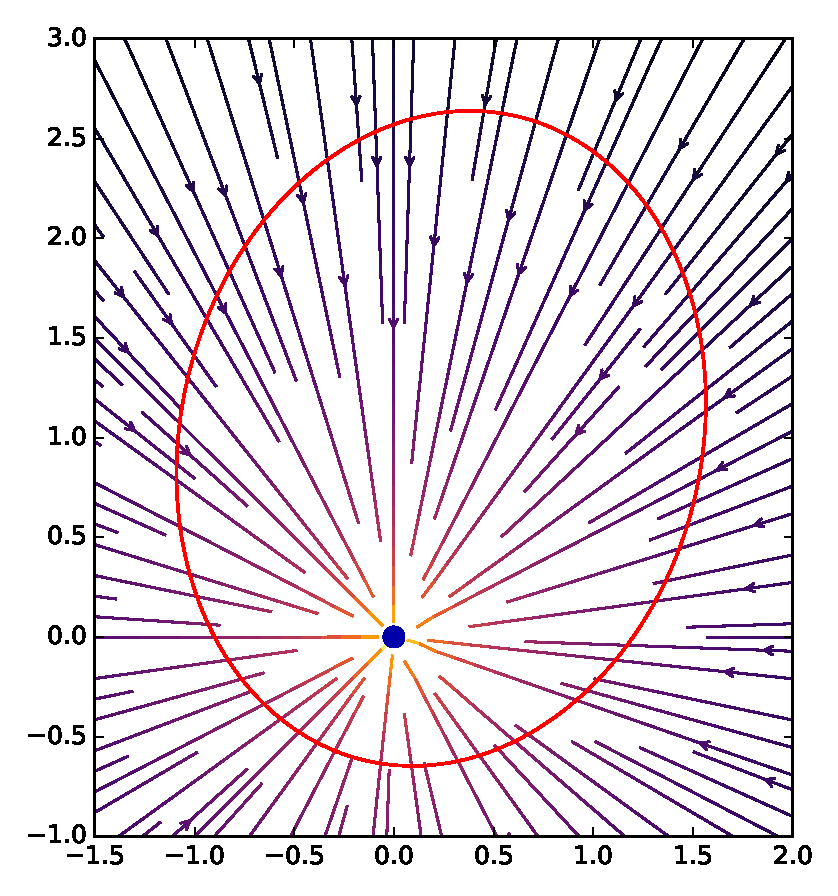
\includegraphics[width=\textwidth]{parts/electrostat/traj_1charge_ellipse.pdf}
	\end{subfigure}
	\begin{subfigure}{0.45\textwidth}
		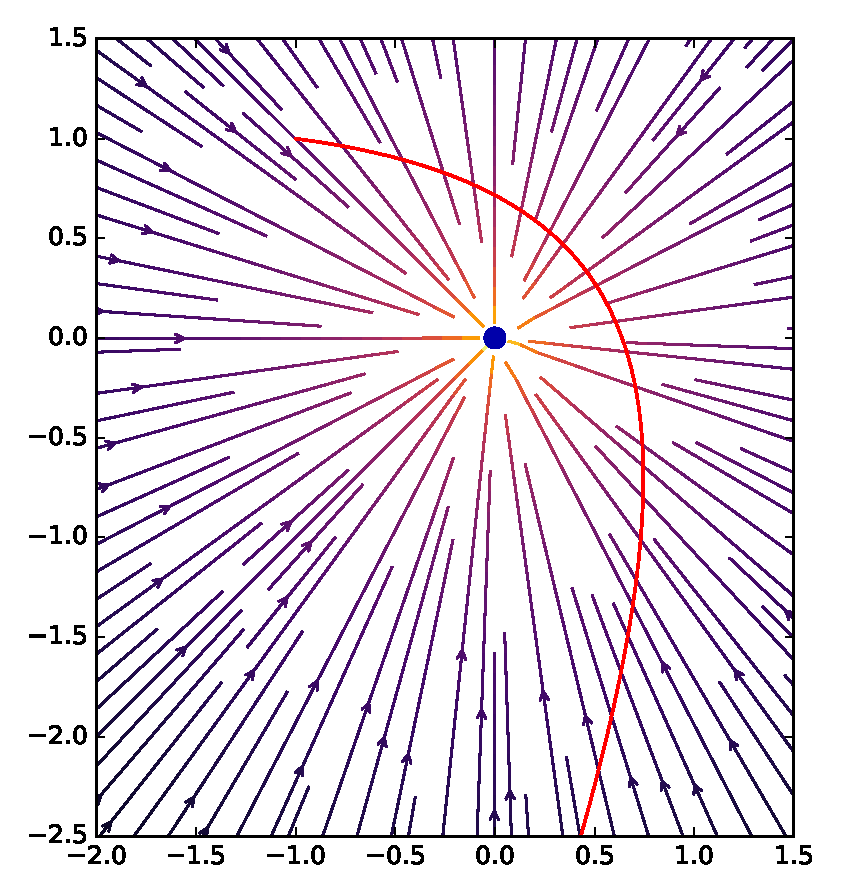
\includegraphics[width=\textwidth]{parts/electrostat/traj_1charge_diverg.pdf}
	\end{subfigure}
	
	\caption{Trajectoires d'une particule dans le champ créé par une charge ponctuelle.}
\end{figure}

\begin{exo}
	On considère deux charges identiques $q$ placées de part et d'autre de l'origine aux points de coordonnées $(-a/2,0)$ et $(a/2,0)$ ($a>0$) respectivement. On aimerait savoir ce qu'il se passe au niveau du champ électrique créé en même temps par ces deux charges.
	
	À l'aide d'un programme \textsf{Python}, on produit la figure suivante:
	
	\begin{center}
		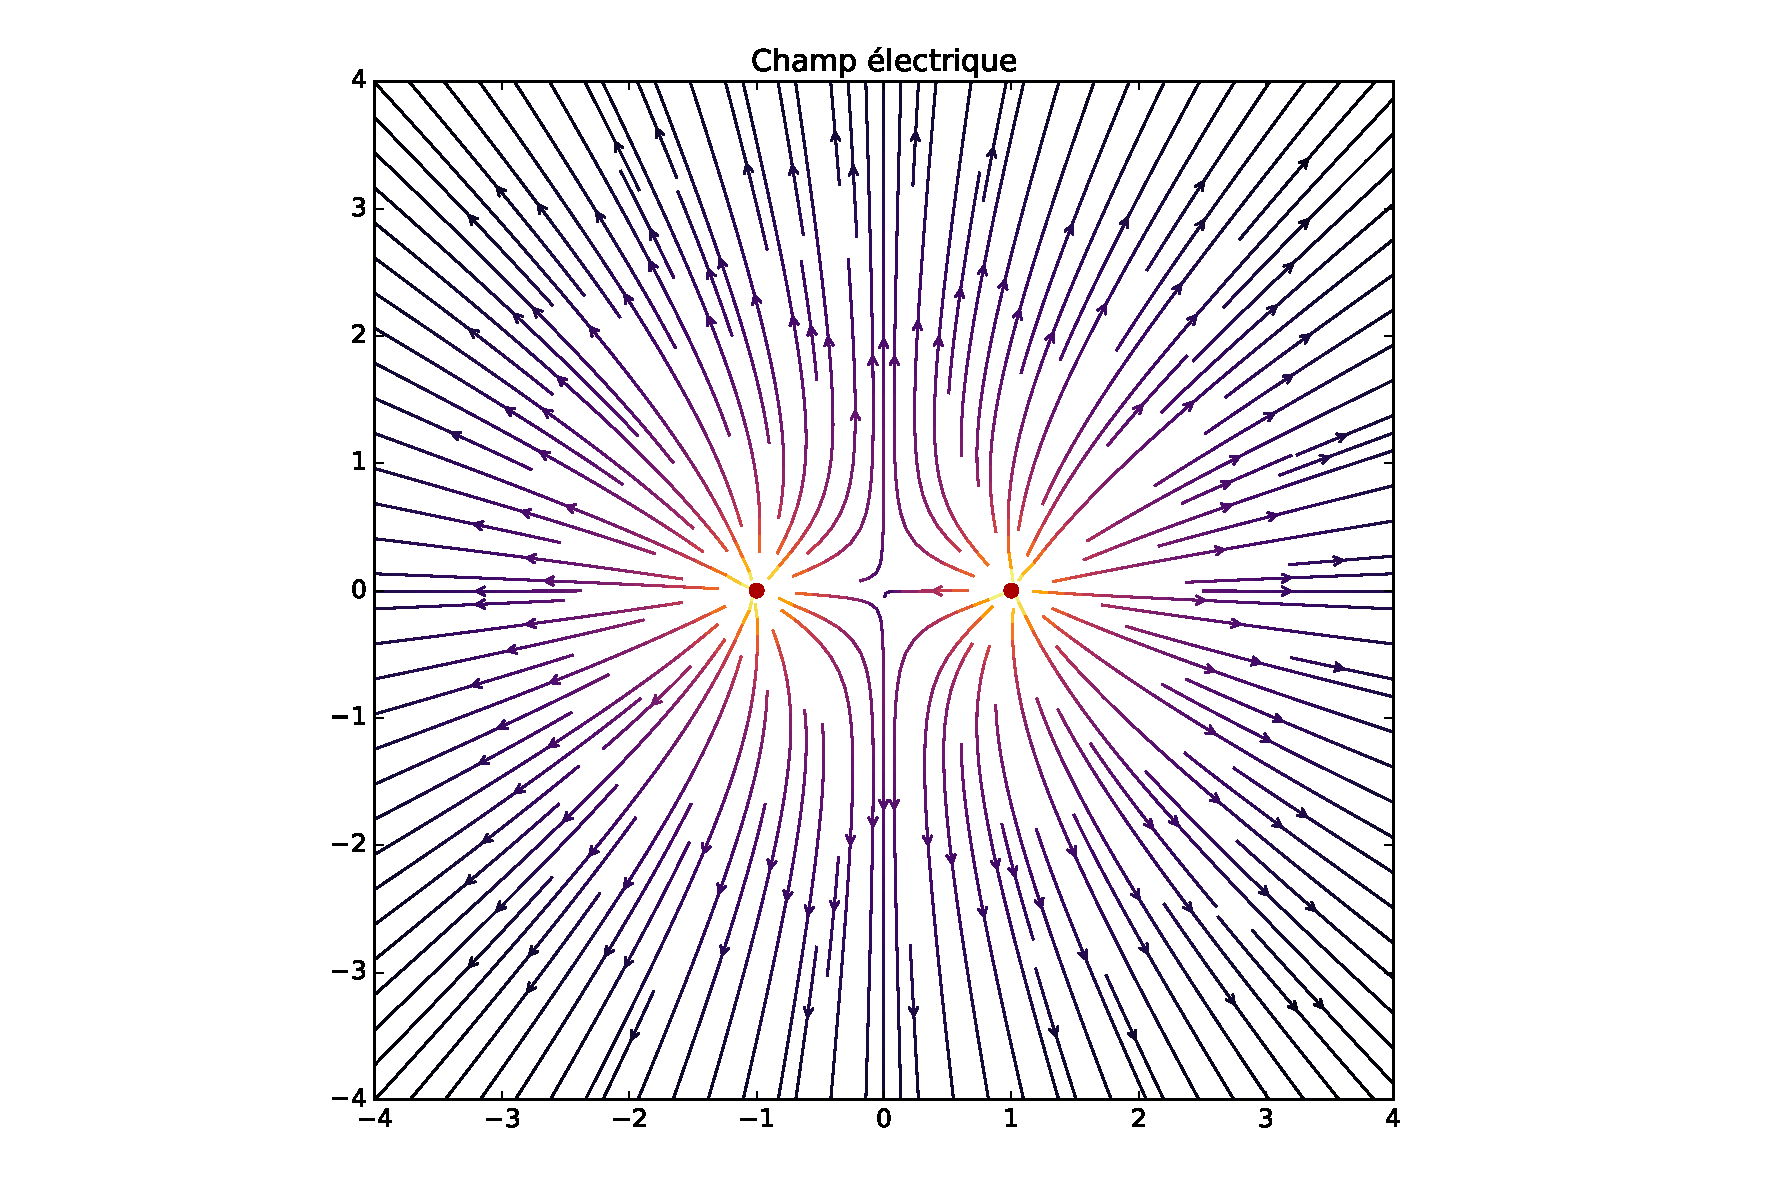
\includegraphics[width=0.9\textwidth]{parts/electrostat/Champ_exo1.pdf}
	\end{center}
	
	\begin{enumerate}
		\item Que dire du champ à l'origine du repère $(0,0)$ ? S'agit-il d'une position d'équilibre stable pour une particule chargée plongée dans le champ ?
		\item Déterminer l'expression du champ électrique dans l'espace privé des points où se situent les charges.
		\item Déterminer une expression simplifiée du champ électrique sur la médiatrice des points $(-a/2,0)$ et $(a/2,0)$ (la droite d'équation $x=0$).
	\end{enumerate}
\end{exo}

\subsection{Dipôle électrique}

\begin{center}
	\textit{<< Pourquoi utilise-t-on si souvent l'eau comme solvant ? >>}
\end{center}

Un dipôle électrique est un système globalement neutre où des charges sont réparties de sorte à ce que que les barycentres des charges négatives et des charges positives ne soient pas confondus. On peut alors se ramener à un système de deux charges opposées $-q$ et $+q$ ($q>0$).

On associe à un dipôle une grandeur vectorielle $\vv{p}$, appelée \textit{moment dipolaire}, et qui prend pour expression
	\[ 
	\vv{p} = qa\vv{u},
	 \]
avec $a$ la distance entre les deux charges et $\vv{u}$ un vecteur unitaire.

\begin{figure}[h]
	\centering
	\begin{tikzpicture}
	\tikzset{dot/.style={circle,fill,inner sep=2pt}};
	
	\node[draw,circle,label={above:$-q$}] (N) at (-1.5,0) {$-$};
	\node[draw,circle,label={above:$+q$}] (P) at (1.5,0) {$+$};
	\draw[color=gray!80,thick] (N)--(P);
	\draw[color=black,thick,->] (N)--(-0.5,0) node[midway,below]{$\vv{u}$};
	
	
	\draw[->,color=red!90,thick] (-1,0.5) -- (1,0.5) node[midway,sloped,above]{$\vv{p}$};
	\end{tikzpicture}
	\caption{Dipôle électrique élémentaire constitué de deux charges $+q$ et $-q$.}
\end{figure}

Bien sûr, comme toute répartition de charges dans l'espace, le dipôle est responsable d'un champ électrostatique, et est lui-même susceptible d'être happé par un champ externe, pouvant induire un déplacement.

\begin{figure}[h]
	\centering
	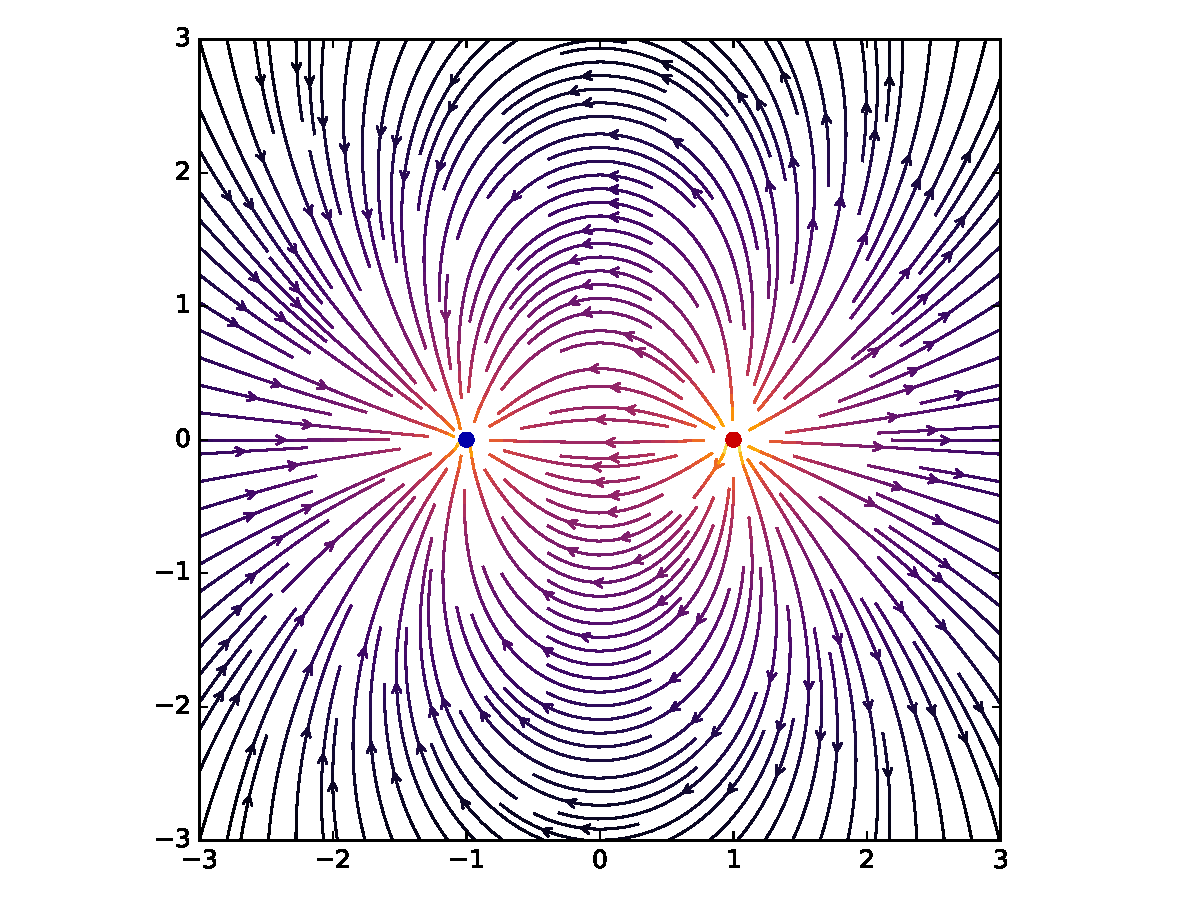
\includegraphics[width=\textwidth]{parts/electrostat/Champ_dipole.pdf}
	\caption{Champ électrique créé par un dipôle électrique : le pôle nord est positif, le pôle sud est négatif.}
\end{figure}

\begin{figure}[h]
	\centering
	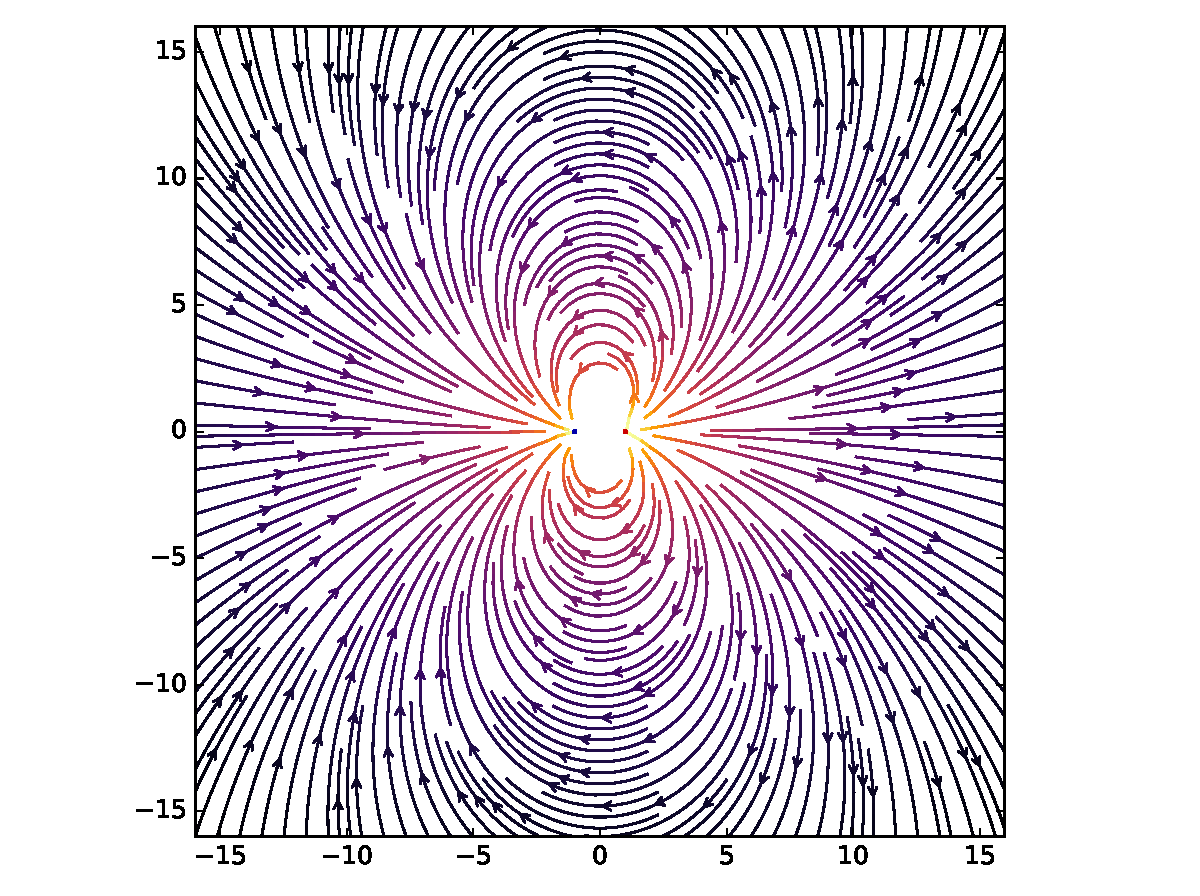
\includegraphics[width=\textwidth]{parts/electrostat/Champ_dipole_loin.pdf}
	\caption{Champ loin du dipôle.}
\end{figure}

On peut montrer que, lorsque soumis à un champ électrostatique $\vv{E}(\vv{r})$, le dipôle électrostatique cherche à minimiser la quantité suivante, appelé \textit{potentiel d'interaction}:
\[ U = -\vv{p}\cdot\vv{E}(\vv{r}), \]
où $\vv{r}$ est le barycentre du dipôle. L'expression donnée est une approximation valable lorsque les variations du champ électrique entre les deux extrémités du dipôle sont négligeables.


En utilisant l'expression du produit scalaire, on obtient
	\[ U = - \norm{\vv{p}}\,\norm{\vv{E}(\vv{r})}\cos\theta, \]
où $\theta$ est l'angle que font $\vv{p}$ et $\vv{E}(\vv{r})$.

Afin de minimiser cette quantité, il faut maximiser $\norm{\vv{E}(\vv{r})}$ et $\cos\theta$. Le dipôle va donc glisser vers là où le champ est plus intense et s'aligner avec lui. 

\begin{rem}
Il se peut que $U$ soit maximal. Dans ce cas, le dipôle restera dans un état d'équilibre dit \textit{instable} : si il bouge (en position ou en angle), il se réalignera sur le champ et sera emporté vers les zones où il est intense.
\end{rem}

\begin{figure}[h]
	\centering
	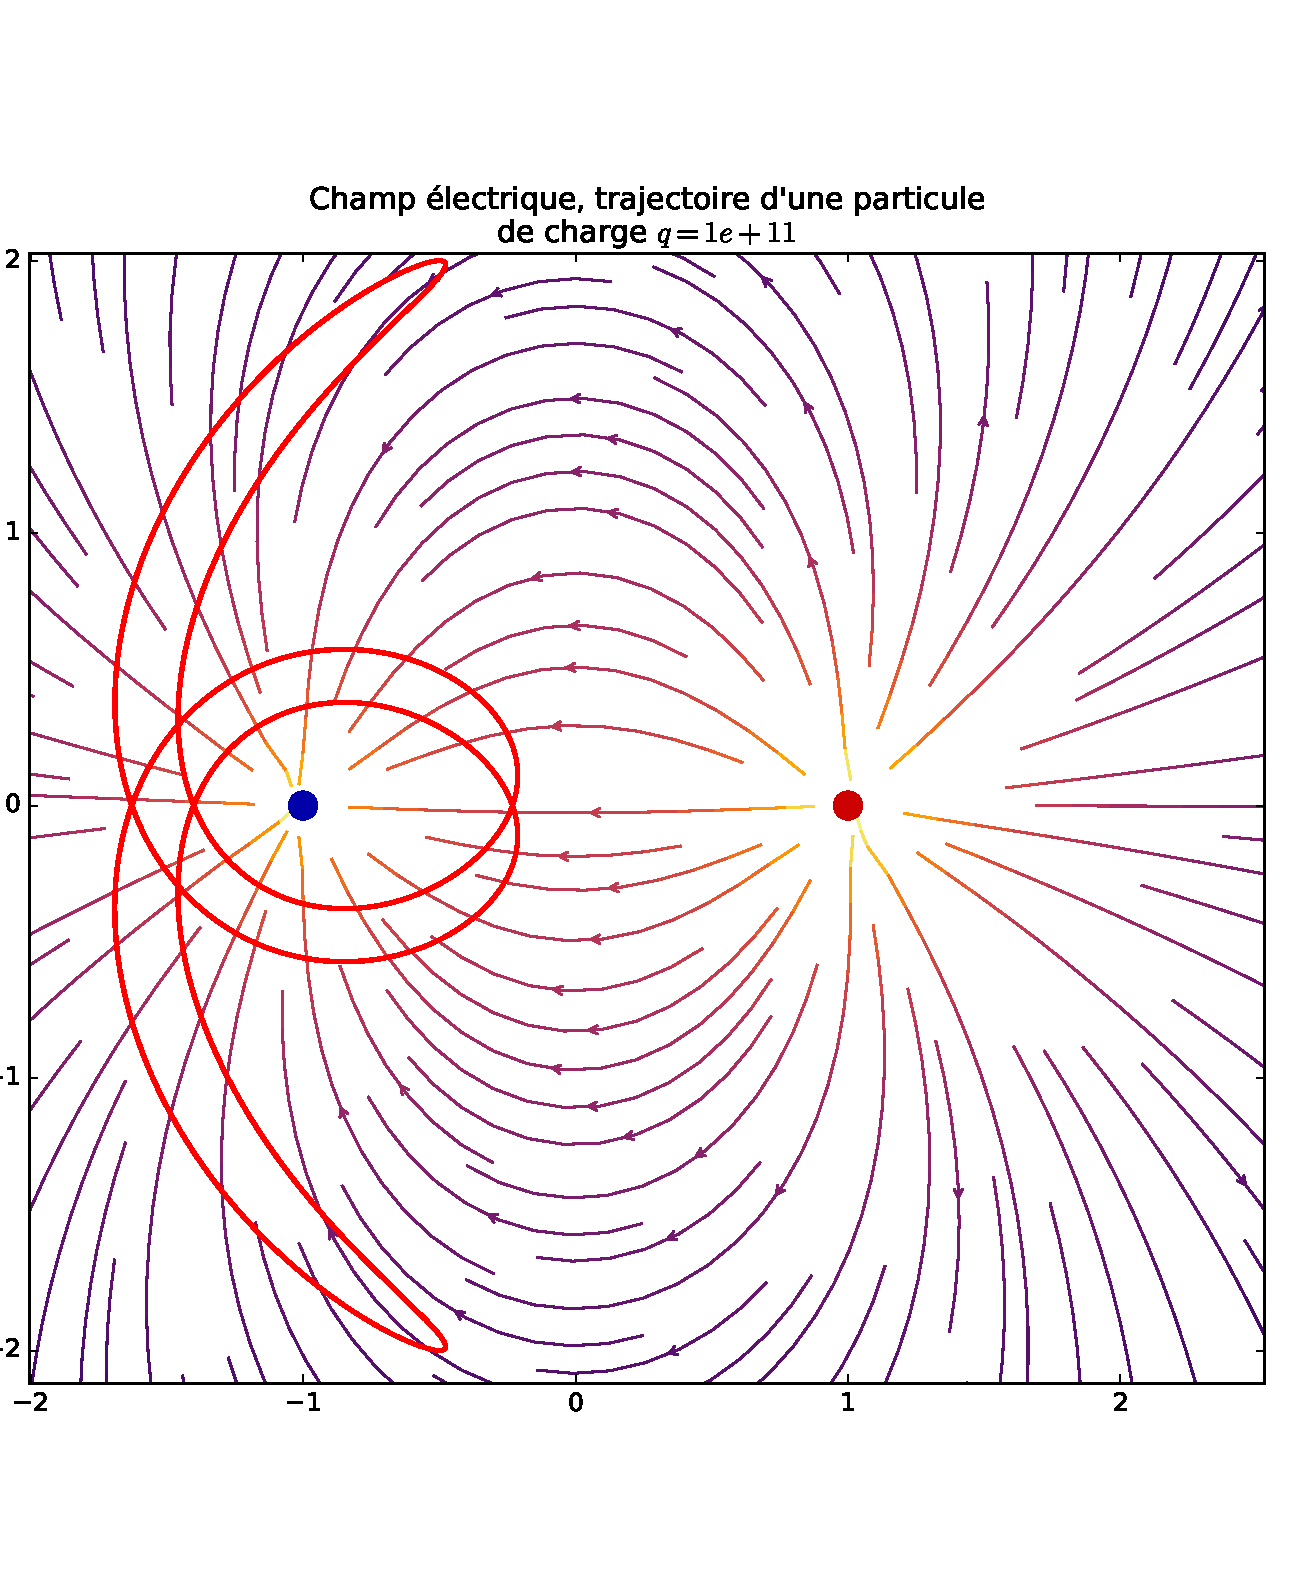
\includegraphics[height=0.9\textheight]{parts/electrostat/traj_x0_-05_2_v0_-1_0.pdf}
	\caption{Trajectoire d'une particule dans le champ créé par un dipôle. Position initiale $\vv{r}_0 = (\num{-0.5};2)$ et vitesse initiale $\vv{v}_0=(-1;0)$. Ici, la trajectoire observée est fermée : le mouvement de la particule est \textit{périodique}. Cela n'arrive pas tout le temps.}
\end{figure}

Une molécule est dite \textit{polaire} lorsque l'électronégativité des éléments la constituant lui donne une structure de dipôle électrique. En effet, le déplacement des électrons intervenant dans des liaisons covalentes faisant apparaître des charges partielles, il se peut que le barycentre de celles qui sont positives et celui de celles qui sont négatives ne soient pas confondus. D'où un dipôle.


Étant donné leur structure originale, où deux charges de signes opposés sont liées, on peut s'attendre à ce que les interactions entre un dipôle et un champ électrique amènent des dimensions nouvelles par rapport à celles entre une charge seule et un champ.

\begin{exo}
	La molécule d'eau est un exemple de molécule polaire. On donne $\delta\approx\num{0.22}$, que la longueur de la liaison de covalence $\mathrm{H}-\mathrm{O}$ est de $\SI{95.8}{\pico\meter}$ et que l'angle entre les deux branches de la molécule est de $\SI{104.5}{°}$.
	\begin{enumerate}
		\item Proposer un modèle de la molécule d'eau comme dipôle électrique. Préciser la distance $d$ entre les barycentres des charges, calculer la norme $p$ du moment dipolaire.
		\item Expliquer pourquoi, quand on approche un peigne fraîchement sorti de ses cheveux d'un filet d'eau, l'eau est déviée malgré le fait que la molécule d'eau est électriquement neutre.
		\item Pourquoi l'eau est-elle, finalement, un bon solvant pour les ions ?
	\end{enumerate}

\begin{figure}[h]
	\centering
	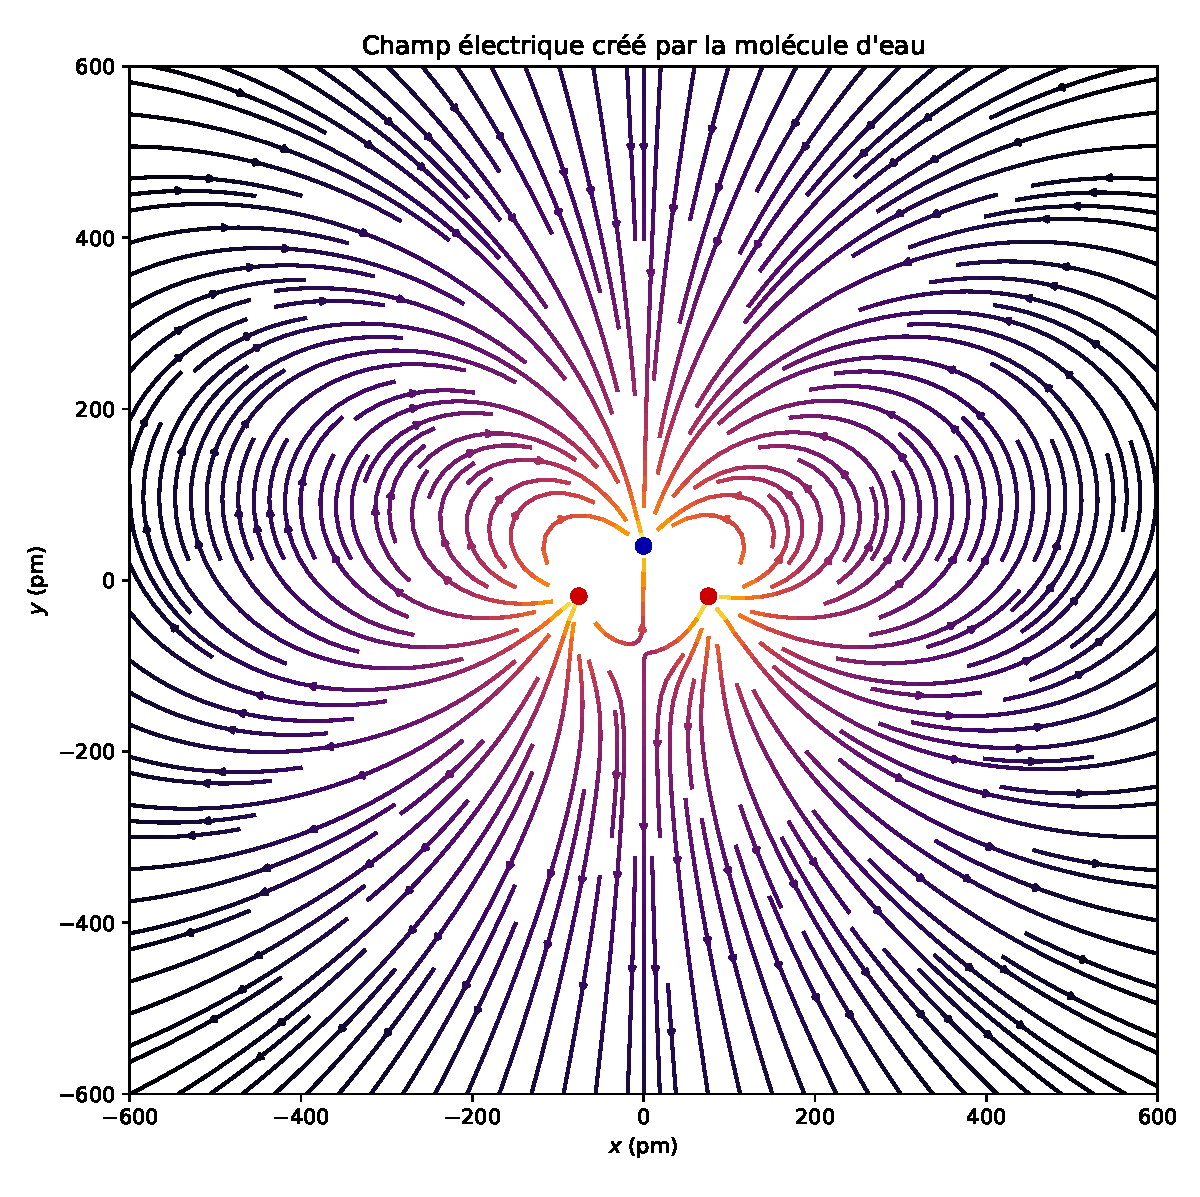
\includegraphics[width=0.96\textwidth]{parts/electrostat/Champ_dipole_eau.pdf}
	\caption{Champ électrique créé par la molécule d'eau.}
\end{figure}

\end{exo}




\end{document}